\chapter{Komponenten}
\label{chap:komponenten}
Ein Expertensystem besteht aus drei Komponenten, wie im~\hyperref[sec:anhang:tutorial_dokument]{Tutorial} unter Kapitel 2 beschrieben.\\
Die Komponenten sind:
\begin{itemize}
    \item Wissensdatenbank: Enthält die Fakten des Problembereiches in formaler Sprache
    \item Inferenz-Maschine: Verarbeitungsmechanismus zum automatischen Ziehen von Schlüssen
    \item Benutzerschnittstelle
\end{itemize}
Wie in~\autoref{ssubsec:vorgehen:grundlagen:technisch} erwähnt, ist die Verwendung von Werkzeugen zur Modellierung einer Ontologie sinnvoll.\\
Dabei gibt es Überschneidungen: \textbf{Komponenten können auch Werkzeuge sein.}

Das folgende Kapitel beschreibt die während dieser Arbeit verwendeten Komponenten und Werkzeuge.

Die Wissensmodellierung sollte ursprünglich mit Hilfe von Apache Stanbol umgesetzt werden, wie unter~\autoref{ssubsec:vorgehen:grundlagen:technisch} erwähnt. Während der Arbeit wurde erkannt, dass diese Technologie für die vorgesehene Aufgabe nur bedingt sinnvoll ist. In Apache Stanbol ist es möglich die modellierte Wissensdomäne zu importieren. Das importierte Modell wird als Ontologie in Form von Tripeln gespeichert. Die Objekte, ihre Eigenschaften sowie Relationen lassen sich jedoch nicht verwalten.

Für Anfragen an die Wissensdatenbank ist eine entsprechende Schnittstelle notwendig. Von Apache Stanbol wird diese Schnittstelle in Form eines SPARQL-Endpoints zur Verfügung gestellt. Der SPARQL-Endpoint nutzt jedoch die ContentHub-Komponente von Apache Stanbol als Datenbasis. Diese stellt nur Wissen zur Verfügung, welches aus angereicherten Inhalten abgeleitet ist. Mittels Ontologien und Regeln werden diese Inhalte angereichert.

Eine aufwendige Recherche ergab: Anderen Datenquellen können für den SPARQL-Endpoint genutzt werden. Dies bedeutet jedoch einen erheblichen Mehraufwand in Form einer eigenen Implementation.

Damit war Apache Stanbol nicht das geeignete Werkzeug für diese Arbeit. Bei weiteren Recherchen wurden weitere Werkzeuge gefunden, welche als Ersatz für Apache Stanbol genutzt werden konnten: \textit{Protégé} der Universität Stanford sowie \textit{Stardog} der Firma Clark \& Parsia.

\section{Stanford Protégé}
\label{sec:komponenten_protege}
Protégé ist eine Entwicklungsumgebung für Ontologien und wurde von den Autoren als \textit{Werkzeug} verwendet. Entwickelt von der Universität Stanford findet es in der Fachwelt häufig Anwendung.\\
Es unterstützt sowohl die Modellierung von Ontologien, wie auch mittels verschiedener Reasoner das Reasoning.

\subsection{Merkmale}
\label{subsec:komponenten_protege_features}
In Protégé können Ontologien in unterschiedlichen Schreibweisen, wie zum Beispiel OWL/XML, Turtle oder RDF/XML eingelesen und abgespeichert werden. Die Dateien tragen immer die Endung ``.owl''. Protégé hält eingelesene Ontologien als Graphstruktur im Speicher~\footnote{\url{http://protegewiki.stanford.edu/wiki/Protege4Features}} und ermöglicht Reasonern den direkten Zugriff auf die Graphstruktur~\footnote{\url{http://protege.stanford.edu/products.php}}.\\
Die Entwicklungsumgebung zeigt verschiedene Ansichten für dieselbe Ontologie. \\
Ausser dem Anlegen und Bearbeiten einer Ontologie können in Protégé (ab Version 5.0.0 Beta-16) SWRL-Regeln verwaltet werden. Diese werden von Protégé direkt in der Ontologie abgelegt.

Durch das SPARQL-Modul bietet Protégé die Möglichkeit Informationen der Ontologie mittels Abfragen zu gewinnen. Ist zusätzlich ein Reasoner-Modul geladen und aktiviert, kann die Umgebung bei Abfragen Inferenzen einbeziehen. Es können verschiedene Reasoner, wie beispielsweise FACT++ oder Pellet genutzt werden (siehe~\ref{subsec:komponenten_reasoner}).

(vgl.~\cite{protegeFeatures})

\subsection{Ansichten}
\label{subsec:komponenten_protege_view}
%Die Benutzerfreundlichkeit von Protégé wird unter Anderem dadurch erreicht, dass verschiedene Sichten auf eine Ontologie geboten werden. 
Protégé bietet benutzerfreundlich mehrere Sichten auf eine Ontologie an.\\
Neben der Entitätsansicht (Entity-View, diese enthält sämtliche Elemente einer Ontologie) existiert für alle Elementtypen wie Klassen, Dateneigenschaften, Objekteigenschaften und Individuen eine eigene Ansicht.

Alle Ansichten sind als Baumstruktur organisiert. Dadurch entsteht eine klare Übersicht. Diese wiederum ermöglicht eine Hierarchie-getreue Abbildung des zu Grunde liegenden XML-Dokumentes.

Protégé bietet weitere Ansichten. Beispielsweise kann der Graph einer Ontologie in der OntoGraf-Ansicht betrachtet werden.

\begin{figure}[H]%[htbp]
    \centering
    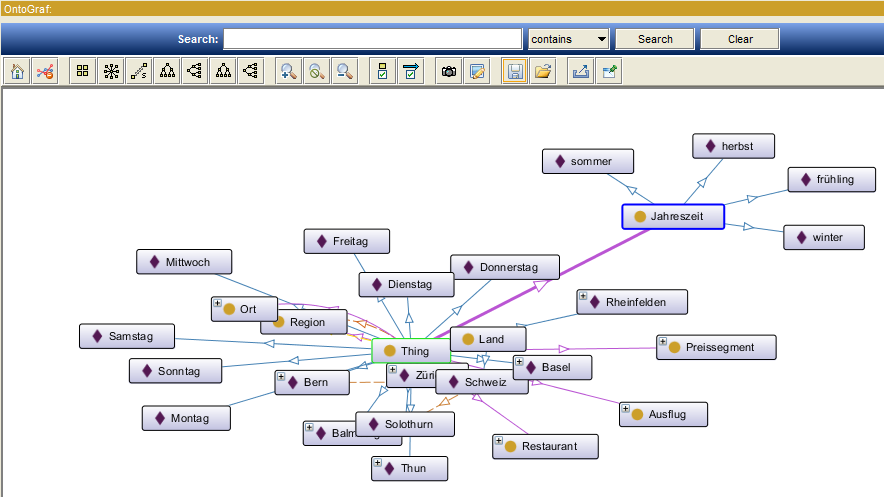
\includegraphics[scale=0.7]{bilder/OntoGraf.png}
    \caption{Beispiel der OntoGraf-Ansicht.\label{fig:kompo:ontograf}\protect\footnotemark}
\end{figure}
\footnotetext{Eigene Darstellung mittels Protégé.}

Schlussfolgerungen werden in allen Ansichten direkt zur Laufzeit des Reasoners bei allen Elementtypen ergänzt.

(vgl.~\cite{protegeView})

\section{Clark \& Parsia Stardog}
\label{sec:komponenten_stardog}
Bei Stardog handelt es sich um eine Graphdatenbank mit Unterstüztung des RDF-Graphenmodelles. Sie bietet den Import und Export von Ontologien in diversen Format an und die Möglichkeit Informationen einer Ontologie mittels SPARQL abzufragen. Des Weiteren unterstützt Stardog die Sprache OWL sowie SWRL-Regeln.\\
Pellet, in Stardog enthalten, bildet eine zentrale Komponente für die Schlussfolgerungen.

Stardog bietet viele Kommunikationsschnittstellen, so z.B. HTTP und SNARL.\\
Programmierschnittstellen sind für zahlreiche Sprachen, so beispielsweise Java, JavaScript oder Python vorhanden.

Stardog unterscheidet drei Versionen der Lizenzierung: Community, Developer und Enterprise. Die Versionen unterscheiden sich durch maximale Anzahl der verwaltbaren Datenbanken und der möglichen Tripel pro Datenbank, Anzahl gleichzeitiger Verbindungen und durch Anzahl Benutzer und Rollen. Je nach gewählter Lizenzierung leistet der Hersteller eine Kundenbetreuung.

(vgl.~\cite{stardogDocu})

\subsection{Reasoner}
\label{subsec:komponenten_reasoner}
Reasoner sind Komponenten,  die Folgerungen von implizitem Wissen zulassen bzw.\ anbieten. Es handelt es sich um eine Art ``Verstehen'' der Maschinen. Ziel ist es, aus explizitem Wissen in Form einer Ontologie implizites Wissen zu gewinnen.

Wie bereits unter~\autoref{ssubsec:vorgehen:grundlagen:technisch} erwähnt, wurde Pellet als Reasoner (Anwendung zum Ziehen von Schlüssen) gewählt. Eine detaillierte Beschreibung von Pellet findet sich im~\hyperref[sec:anhang:tutorial_dokument]{Tutorial} unter Abschnitt 6.4.

\subsection{Konkrete Anwendung der Komponenten zur Modellierung der Ontologie}
\label{subsec:komponenten_anwendung}
Im Laufe der Arbeit hat sich herausgestellt, dass das Schlussfolgern in Protégé nicht einwandfrei funktioniert. Gewisse SPARQL-Anfragen wurden nicht erwartungsgemäss beantwortet.

Da sowohl Protégé als auch Stardog dieselbe Komponente für Schlussfolgerungen (den Pellet-Reasoner) verwenden, muss es sich bei dem Fehlverhalten um einen Fehler bei der Aufbereitung der Abfragen handeln.

In Protégé existiert zudem keine HTTP-Schnittstelle. Es existiert zwar eine Programmierschnittstelle mit welcher eine HTTP-Schnittstelle geschaffen werden kann, dies wurde aber aus zeitlichen Gründen verworfen.

Angesichts der Funktionsstörung und mangelnder HTTP-Schnittstelle, wurde die Ontologie in Protégé erstellt und bearbeitet. Die Weiterverarbeitung der Ontolgie erfolgte mittels Stardog, da Stardog die SPARQL-Anfragen korrekt beantwortet und ausserdem eine HTTP- und REST-Schnittstelle bietet.

Dafür musste in Stardog eine neue Datenbank erstellt werden. In diese wurde die mittels Protégé vorbereitete Ontologie im RDF/XML-Format eingespielt.

Stardog bietet bei der Verwendung des Reasoners mehr Möglichkeiten als die anderen Werkzeuge (wie zum Beispiel Protégé). Schlussfolgerungen werden mittels einer Kombination von RDFS-, QL-, RL- und EL-Axiomen sowie zusätzlich SWRL-Regeln gezogen. Details finden sich unter der Webseite~\href{http://docs.stardog.com/\#_reasoning_levels}{docs.stardog.com}\footnote{\url{http://docs.stardog.com/\#_reasoning_levels}}.


Durch die Kombination der Werkzeuge Protégé und Stardog konnte eine zuverlässige Modellierung und Verwendung der Ontologie erreicht werden.

\section{Benuzteroberfläche}
\label{sec:komponenten:ember}
Ein Teil der Aufgabe bestand darin, eine möglichst benutzerfreundliche Schnittstelle zwischen Mensch und System zu entwickeln.\\
Als Schnittstelle haben die Autoren eine Webapplikation zur Reiseplanung entwickelt, wie im~\autoref{sec:loesung_gui} ausgeführt. Diese ermöglicht das Planen einer Reise mit Hilfe eines Assistenten. Der Benutzer kann die gewünschten Reisekriterien auswählen und erhält schliesslich eine Auswahl an Reiseobjekten, welche seinen Kriterien entsprechen.

\subsection{Komponenten der Benutzeroberfläche}
\label{subsec:komponenten:gui:komponenten}
Folgende Komponenten wurden zur Umsetzung der Benutzeroberfläche gewählt:
\begin{itemize}
    \item \textit{Vagrant}\footnote{\url{http://www.vagrantup.com}}\\
        Virtualisierungslösung
    \item \textit{nginx}\footnote{\url{https://nginx.org}}\\
        Webserver
    \item \textit{Ember.js}\footnote{\url{http://emberjs.com}}\\
        Applikations-Framework
    \item \textit{Bootstrap}\footnote{\url{http://getbootstrap.com}}\\
        HTML-, CSS- und JavaScript-Framework von Twitter
\end{itemize}
(Die Auswahl erfolgte aufgrund beruflicher Erfahrungen der Autoren.)

\subsubsection{Vagrant}
\label{ssubsec:komponenten:gui:komponenten:vagrant}
Bei Vagrant handelt es sich um ein Werkzeug zur Erstellung von vollständigen Entwicklungsumgebungen basierend auf Virtualisierung (vgl.~\cite{vagrant}). Details dazu finden sich unter der Webseite~\href{http://www.vagrantup.com/about.html}{vagrantup.com}\footnote{\url{http://www.vagrantup.com/about.html}}.

In der vorliegend Arbeit wurde Vagrant zur Bereitstellung einer (virtuellen) Entwicklungsumgebung genutzt. Dabei wird die eigentliche Anwendung von der Entwicklungsumgebung getrennt. Dadurch kann die Entwicklungsumgebung jederzeit mittels weniger Befehle wieder neu aufgebaut werden.

\subsubsection{nginx}
\label{ssubsec:komponenten:gui:komponenten:nginx}
nginx (``engine x'' ausgesprochen) ist ein freier open-source Webserver. Seine Stärken liegen unter anderem  auf hoher Leistung, hoher Nebenläufigkeit und geringem Speicherverbrauch. Er ist der am zweithäufigsten eingesetzte Webserver (vgl.~\cite{nginx}).

nginx wurde innerhalb der (virtuellen) Entwicklungsumgebung zur Bereitstellung der Applikation genutzt. So kann die Applikation innerhalb eines Rechners wie eine externe Webseite angesprochen werden.

\subsubsection{Ember.js}
\label{ssubsec:komponenten:gui:komponenten:emberjs}
Ember.js ist ein clientseitiges open-source Framework zur Erstellung von Webapplikationen. Es baut auf dem Model-View-Controller (MVC) Softwarearchitektur-Muster auf. Es erlaubt die Erstellung von skalierbaren Anwendungen mittels einer einzigen Datei und bietet dabei deklarative Datenbindung, dynamische Eigenschaften, automatisch aktualisierte Templates sowie eine Zustandsverwaltung der Applikation mittels einer Router-Komponente (vgl.~\cite{ember}).

Ember.js wurde für die Umsetzung der Applikationslogik der Benutzeroberfläche eingesetzt.

\subsubsection{Bootstrap}
\label{ssubsec:komponenten:gui:komponenten:bootstrap}
Bootstrap der Firma Twitter ist eine Sammlung von Werkzeugen um Webseiten und Webapplikationen zu erstellen. Bootstrap bietet unter anderem verschiedene, auf HTML und CSS basierende Vorlagen für Typographie, Formulare, Schaltflächen und Navigation (vgl.~\cite{bootstrap}).

Bootstrap wurde zur grafischen Gestaltung der Benutzeroberfläche eingesetzt.

\subsection{Architektur}
\label{subsec:komponenten:gui:architektur}
\begin{figure}[H]
    \centering \rotatebox{0}{\scalebox{0.5}[0.5]{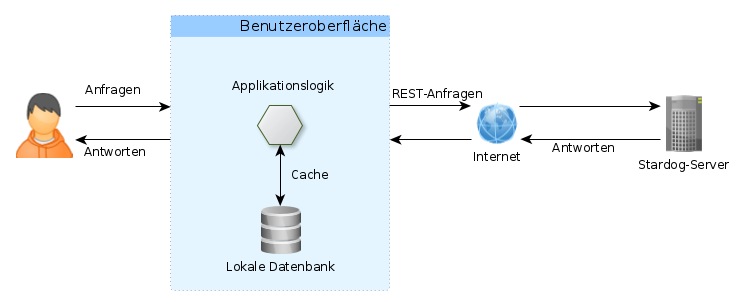
\includegraphics{bilder/architektur_gui.png}}}
    \caption{Architektur der Benutzeroberfläche\label{fig:architektur:gui}\protect\footnotemark}
\end{figure}
\footnotetext{Eigene Darstellung mittels yEd.}

Die obenstehende Abbildung~\ref{fig:architektur:gui} zeigt die Architektur der Benutzeroberfläche, bestehend aus einem Frontend und einem Backend. Mit Frontend ist die Applikation selbst (Benutzeroberfläche) gemeint, mit Backend der Stardog-Server.

Die Applikation besteht aus \textit{Modellen}, \textit{Ansichten} und \textit{Routen}.

\textit{Modelle} sind \textit{Reisen}, \textit{Dateneigenschaften} und \textit{Objektrelationen}.\\
\hangindent=1.5cm Das \textit{Modell} \textit{Reise} entspricht \textit{Individuen}, das \textit{Modell} \textit{Dateneigenschaft} \textit{DataProperties} und\\
das \textit{Modell} \textit{Objektrelation} den \textit{ObjectProperties} der Ontologie.

\textit{Routen} definieren, entsprechend ihrem Namen, den Ablauf der Applikation.\\
\hangindent=1.5cm \textit{Welcome}-Route ist der Einstieg der Applikation. Von der \textit{Welcome}-Route aus werden die \textit{Routen} \textit{Step1}, \textit{Step2} und \textit{Step3} nacheinander in Form eines Schritt-für-Schritt-Assistenten durchlaufen.\\
In Schritt 1 wird die Art der Ausflüge gewählt.\\
In Schritt 2 werden die \textit{Dateneigenschaften} sowie die \textit{Objektrelationen} pro zuvor gewählter Art der Ausflüge gewählt.\\
Schritt 3 gibt alle Instanzen zurück, welche den gewählten Kriterien entsprechen.\\
\\
Da in Schritt 1 nur bestimmte Individuen der Ontologie angezeigt werden sollen, wurden in der Ontologie diese Individuen mit der \textit{Dateneigenschaft} ``reise'' gekennzeichnet. Dadurch beschränkt sich die Abfrage von Schritt 1 nur auf diese Individuen.

Die \textit{Ansichten} kombinieren die Gestaltung (das Layout) der Seite mit der Ansicht der aktuellen Route.

Die gewählte Graphdatenbank Stardog bietet externen Zugriff via REST-Protokoll. Das gewählte Framework Ember.js bietet REST-Unterstützung via REST-Adapter an. Der REST-Adapter implementiert standardmässig Lesen und Schreiben einer REST-Schnittstelle.

Da das Ziel der Arbeit nicht eine vollständige Umsetzung (Lesen und Schreiben) der Ontologie war, wurde der Zugriff auf die Datenbank nur lesend implementiert. Dadurch kann die umgesetzte Applikation und somit der Benutzer Daten der Ontologie nur lesen (und nicht ändern). Daher musste das Standardverhalten des REST-Adapters von Ember.js durch Nutzung der lokalen Datenbank von Ember.js umgangen werden.

Beim initialen Aufruf der Applikation wird die gesamte Ontologie via REST-Protokoll vom Server abgerufen und nur in der lokalen Datenbank von Ember.js in Form der \textit{Modelle} abgelegt. Damit der Benutzer beim initialen Aufruf der Applikation nicht auf den Datenaustausch warten muss und die Applikation nicht blockiert wird, findet der Datenaustausch asynchron statt. Trotz im  Hintergrund laufender Anfragen kann die Applikation benützt werden. Dabei werden die \textit{Modelle} an die \textit{Ansicht} gebunden. Das heisst, erhält die Applikation Daten eines Modells, wird automatisch dessen \textit{Ansicht} dargestellt bzw.\ aktualisiert.
